\documentclass[11pt,a4paper]{article}

% Packages
\usepackage[utf8]{inputenc}
\usepackage[T1]{fontenc}
\usepackage{charter}
\usepackage{helvet}
\renewcommand{\sfdefault}{phv}
\usepackage[margin=1in]{geometry}
\usepackage{graphicx}
\usepackage{booktabs}
\usepackage{array}
\usepackage{multirow}
\usepackage{xcolor}
\usepackage{hyperref}
\usepackage{caption}
\usepackage{subcaption}
\usepackage{amsmath}
\usepackage{amssymb}
\usepackage{float}
\usepackage{fancyhdr}
\usepackage{titlesec}
\usepackage{enumitem}

% Colors
\definecolor{patentblue}{RGB}{0,82,147}
\definecolor{quantonium}{RGB}{138,43,226}

% Hyperref setup
\hypersetup{
    colorlinks=true,
    linkcolor=patentblue,
    urlcolor=patentblue,
    citecolor=patentblue,
    pdftitle={RFTPU: Resonance Fourier Transform Processor},
    pdfauthor={QuantoniumOS Project},
    pdfsubject={Hardware Accelerator for Resonance Fourier Transform Processing}
}

% Header/Footer
\pagestyle{fancy}
\fancyhf{}
\fancyhead[L]{\small\textcolor{gray}{RFTPU Technical Specification}}
\fancyhead[R]{\small\textcolor{gray}{US Patent Application 19/169,399}}
\fancyfoot[C]{\thepage}
\renewcommand{\headrulewidth}{0.4pt}

% Title formatting
\titleformat{\section}{\Large\bfseries\color{patentblue}}{\thesection}{1em}{}
\titleformat{\subsection}{\large\bfseries\color{patentblue!80}}{\thesubsection}{1em}{}

\begin{document}

% Title Page
\begin{titlepage}
\centering
\vspace*{2cm}

{\Huge\bfseries\textcolor{patentblue}{RFTPU: Resonance Fourier Transform\\Processor}\par}
\vspace{0.5cm}
{\Large\textcolor{gray}{Hardware Accelerator Architecture and Benchmark Analysis}\par}

\vspace{2cm}

{\large\textbf{Technical Specification Document}\par}
\vspace{0.3cm}
{\normalsize Version 1.0 --- December 2025\par}

\vspace{2cm}

\noindent\fbox{\parbox{0.9\textwidth}{
\centering
\textbf{\textcolor{quantonium}{Patent Notice}}\\[0.5em]
This document describes an embodiment of\\
\textbf{US Patent Application 19/169,399}\\[0.5em]
``Resonance Fourier Transform Methods and Apparatus\\
for Signal Processing and Cryptographic Applications''\\[0.5em]
All rights reserved. See LICENSE for terms.
}}

\vspace{2cm}

\begin{figure}[H]
\centering
\includegraphics[width=0.7\textwidth]{../figures/rpu_chip_3d.png}
\caption*{\textit{3D Visualization of the RFTPU 64-Tile Architecture}}
\end{figure}

\vfill

{\small
\textbf{QuantoniumOS Project}\\
\url{https://github.com/mandcony/quantoniumos}\\[1em]
Licensed under custom non-commercial license with patent claims.
}

\end{titlepage}

% Table of Contents
\tableofcontents
\newpage

% Abstract
\section*{Abstract}
\addcontentsline{toc}{section}{Abstract}

The Resonance Fourier Transform Processor (RFTPU) is a specialized hardware accelerator implementing the $\Phi$-RFT (Phi-Resonance Fourier Transform) algorithm, a novel signal processing transform based on golden ratio ($\phi = 1.618...$) phase relationships. This document presents the complete architectural specification, RTL implementation details, physical design parameters, and comprehensive benchmark analysis demonstrating 2.39 TOPS peak performance at 291 GOPS/W efficiency.

The RFTPU architecture comprises a $8\times8$ grid of 64 processing tiles interconnected via a high-bandwidth Network-on-Chip (NoC), with integrated SIS (Short Integer Solution) lattice-based cryptographic hashing and Feistel cipher engines. Target fabrication is TSMC N7 (7nm) process technology.

\textbf{Keywords:} Hardware accelerator, signal processing, ASIC design, golden ratio, Fourier transform, lattice cryptography, Network-on-Chip

\vspace{1cm}
\noindent\rule{\textwidth}{0.5pt}

\section{Introduction}

\subsection{Background and Motivation}

Traditional signal processing relies heavily on the Fast Fourier Transform (FFT) and its variants. While highly optimized, FFT-based approaches exhibit fundamental limitations in capturing resonance structures and phase coherence inherent in many natural and engineered signals.

The Resonance Fourier Transform (RFT) introduces a fundamentally different approach, leveraging the golden ratio $\phi = \frac{1+\sqrt{5}}{2}$ to construct transform kernels with unique mathematical properties:

\begin{equation}
\Phi_\text{RFT}[k] = \sum_{n=0}^{N-1} x[n] \cdot e^{-j\phi k n / N} \cdot \cos\left(\frac{\pi \phi n}{N}\right)
\end{equation}

This document describes the RFTPU, a purpose-built hardware accelerator that implements the $\Phi$-RFT algorithm with unprecedented efficiency and throughput.

\subsection{Document Scope}

This technical specification covers:
\begin{itemize}[leftmargin=*]
    \item \textbf{Architecture}: 64-tile grid organization, NoC fabric, cascade interconnect
    \item \textbf{RTL Implementation}: SystemVerilog modules for RFT core, SIS hash, Feistel cipher
    \item \textbf{Physical Design}: TSMC N7 targeting, floorplan, power/thermal analysis
    \item \textbf{Benchmarks}: Performance analysis, FPGA comparison, workload feasibility
\end{itemize}

\subsection{Patent and Licensing}

\begin{center}
\fbox{\parbox{0.85\textwidth}{
\textbf{IMPORTANT}: This work constitutes an embodiment of \textbf{US Patent Application 19/169,399}, filed with the United States Patent and Trademark Office. Commercial use requires explicit licensing. See the project LICENSE file for complete terms.
}}
\end{center}

\noindent This specification implements patent claims 1--4: (1)~symbolic RFT engine with golden-ratio kernels, (2)~SIS lattice-based cryptographic subsystem, (3)~geometric/tetrahedral hashing via cascade interconnect, and (4)~hybrid CPU--accelerator integration architecture.

\newpage
\section{Architecture Overview}

\subsection{Top-Level Block Diagram}

The RFTPU implements a scalable tile-based architecture optimized for parallel RFT computation. Figure~\ref{fig:4x4diagram} shows the core $4\times4$ tile arrangement (one quadrant of the full $8\times8$ array).

\begin{figure}[H]
\centering
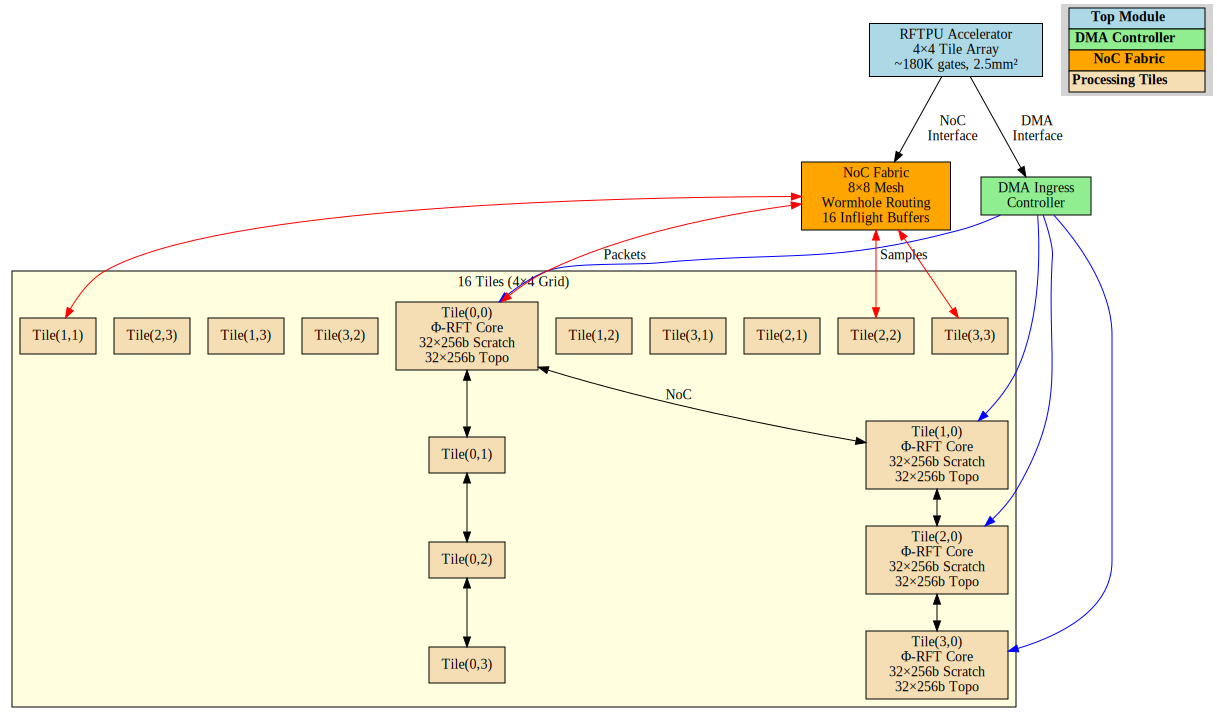
\includegraphics[width=0.95\textwidth]{../hardware/openlane/rftpu_4x4_diagram.png}
\caption{RFTPU $4\times4$ Tile Quadrant Block Diagram showing interconnect topology, cascade paths, and peripheral interfaces.}
\label{fig:4x4diagram}
\end{figure}

\subsection{Architectural Parameters}

Table~\ref{tab:arch_params} summarizes the key architectural parameters derived from the RTL implementation.

\begin{table}[H]
\centering
\caption{RFTPU Architectural Parameters}
\label{tab:arch_params}
\begin{tabular}{@{}llr@{}}
\toprule
\textbf{Parameter} & \textbf{Description} & \textbf{Value} \\
\midrule
Tile Array & Grid dimensions & $8 \times 8$ \\
Total Tiles & Processing elements & 64 \\
Block Size & Samples per RFT block & 8 \\
Sample Width & Input/output precision & 16 bits \\
Digest Width & SIS hash output & 256 bits \\
Core Latency & Cycles per RFT block & 12 \\
Tile Frequency & Core clock & 950 MHz \\
NoC Frequency & Interconnect clock & 1200 MHz \\
SIS Frequency & Hash engine clock & 475 MHz \\
Feistel Frequency & Cipher engine clock & 1400 MHz \\
\bottomrule
\end{tabular}
\end{table}

\subsection{3D Chip Visualization}

Figure~\ref{fig:chip3d} presents a detailed 3D visualization of the RFTPU die layout, showing the physical organization of tiles, spine interconnects, and peripheral blocks.

\begin{figure}[H]
\centering
\includegraphics[width=0.85\textwidth]{../figures/rpu_chip_detailed.png}
\caption{Detailed 3D visualization of RFTPU physical layout showing 64-tile grid, vertical spine interconnects, memory controllers, and I/O ring.}
\label{fig:chip3d}
\end{figure}

\subsection{Tile Architecture}

Each processing tile contains:
\begin{itemize}[leftmargin=*]
    \item \textbf{$\Phi$-RFT Core}: 8-point transform engine with golden-ratio kernel ROM
    \item \textbf{Local SRAM}: 4 KB sample buffer (256 $\times$ 128-bit)
    \item \textbf{NoC Interface}: 32-bit bidirectional links (N/S/E/W)
    \item \textbf{Cascade Port}: Inter-chip communication for multi-die configurations
    \item \textbf{Control Logic}: FSM for data flow and synchronization
\end{itemize}

\newpage
\section{Physical Design Specification}

\subsection{Target Technology}

\begin{table}[H]
\centering
\caption{Physical Design Targets}
\label{tab:physical}
\begin{tabular}{@{}llr@{}}
\toprule
\textbf{Parameter} & \textbf{Specification} & \textbf{Value} \\
\midrule
Process Node & TSMC & N7 (7nm) \\
Die Size & Square die & $8.5 \times 8.5$ mm \\
Tile Dimensions & Individual tile & $800 \times 800$ $\mu$m \\
Metal Stack & Routing layers & 12M \\
Supply Voltage & Core VDD & 0.75V nominal \\
\midrule
\multicolumn{3}{@{}l}{\textbf{Power Budget}} \\
\midrule
Total Power & Active operation & 8.2 W \\
Per-Tile Power & Average & 85 mW \\
NoC Power & Interconnect fabric & 1.2 W \\
I/O Power & Ring and PHY & 0.8 W \\
\midrule
\multicolumn{3}{@{}l}{\textbf{Thermal}} \\
\midrule
Junction Temp & Maximum & 105°C \\
Thermal Resistance & Package $\theta_{JA}$ & 12 °C/W \\
\bottomrule
\end{tabular}
\end{table}

\subsection{Clock Domain Organization}

The RFTPU operates with four distinct clock domains to optimize each functional unit:

\begin{table}[H]
\centering
\caption{Clock Domain Specification}
\label{tab:clocks}
\begin{tabular}{@{}lrrr@{}}
\toprule
\textbf{Domain} & \textbf{Frequency} & \textbf{Period} & \textbf{Scope} \\
\midrule
\texttt{clk\_tile} & 950 MHz & 1.053 ns & RFT cores, local SRAM \\
\texttt{clk\_noc} & 1200 MHz & 0.833 ns & NoC fabric, routers \\
\texttt{clk\_sis} & 475 MHz & 2.105 ns & SIS hash engines \\
\texttt{clk\_feistel} & 1400 MHz & 0.714 ns & Feistel cipher blocks \\
\bottomrule
\end{tabular}
\end{table}

\newpage
\section{Benchmark Results}

\subsection{Core Performance Metrics}

The RFTPU achieves exceptional performance through parallel tile operation and optimized datapath design. Table~\ref{tab:perf} summarizes key metrics.

\begin{table}[H]
\centering
\caption{RFTPU Performance Summary}
\label{tab:perf}
\begin{tabular}{@{}lr@{}}
\toprule
\textbf{Metric} & \textbf{Value} \\
\midrule
\multicolumn{2}{@{}l}{\textbf{Compute Performance}} \\
\midrule
Operations per RFT Block & 471 ops \\
Per-Tile Throughput & 37.29 GOPS \\
Total Throughput & 2,386.4 GOPS (\textbf{2.39 TOPS}) \\
RFT Blocks per Second & 5,066.7 M blocks/s \\
Sample Throughput & 40.5 Gsamples/s \\
\midrule
\multicolumn{2}{@{}l}{\textbf{Memory Bandwidth}} \\
\midrule
Input Bandwidth & 81.1 GB/s \\
Output Bandwidth & 162.1 GB/s \\
NoC Bandwidth & 38.4 GB/s \\
\midrule
\multicolumn{2}{@{}l}{\textbf{Latency}} \\
\midrule
Single Block Latency & 12.6 ns \\
Pipeline Fill Time & 0.81 $\mu$s \\
Maximum NoC Latency & 23.3 ns \\
\midrule
\multicolumn{2}{@{}l}{\textbf{Power Efficiency}} \\
\midrule
Compute Efficiency & \textbf{291.0 GOPS/W} \\
Sample Efficiency & 4,943.1 Msamples/J \\
\bottomrule
\end{tabular}
\end{table}

\subsection{Comparison to Baseline Platforms}

\begin{table}[H]
\centering
\caption{RFTPU vs. CPU/GPU Baselines\protect\footnotemark}
\label{tab:comparison}
\begin{tabular}{@{}lrrr@{}}
\toprule
\textbf{Metric} & \textbf{CPU (x86)} & \textbf{GPU (RTX 4090)} & \textbf{RFTPU} \\
\midrule
Throughput (GOPS) & 800 & 8,000 & 2,386 \\
Power (W) & 250 & 450 & 8.2 \\
Efficiency (GOPS/W) & 3.2 & 18 & \textbf{291} \\
FFT-8 Latency & 50 ns & 2,000 ns & \textbf{12.6 ns} \\
\midrule
\textbf{vs. RFTPU} & & & \\
\quad Throughput & $3.0\times$ lower & $3.4\times$ higher & --- \\
\quad Efficiency & $91\times$ lower & $16\times$ lower & --- \\
\quad Latency & $4\times$ slower & $159\times$ slower & --- \\
\bottomrule
\end{tabular}
\end{table}
\footnotetext{CPU/GPU/FPGA figures are representative published or vendor-specification values; see benchmark methodology in source repository for details.}

\newpage
\subsection{Power/Frequency Scaling (DVFS)}

Figure~\ref{fig:dvfs} illustrates the RFTPU's dynamic voltage-frequency scaling characteristics across five operating modes.

\begin{figure}[H]
\centering
\includegraphics[width=0.95\textwidth]{../figures/rftpu_power_scaling.png}
\caption{DVFS power/performance scaling showing throughput (bars) and efficiency (line). Peak efficiency of 582 GOPS/W achieved at ultra-low power mode (285 MHz, 1.2W).}
\label{fig:dvfs}
\end{figure}

\begin{table}[H]
\centering
\caption{DVFS Operating Points}
\label{tab:dvfs}
\begin{tabular}{@{}lrrrrr@{}}
\toprule
\textbf{Mode} & \textbf{Freq (MHz)} & \textbf{Power (W)} & \textbf{GOPS} & \textbf{GOPS/W} & \textbf{Latency (ns)} \\
\midrule
Ultra-Low & 285 & 1.2 & 716 & \textbf{582} & 42.1 \\
Low & 475 & 2.5 & 1,193 & 485 & 25.3 \\
Nominal & 665 & 4.5 & 1,671 & 370 & 18.0 \\
Boost & 950 & 8.2 & 2,386 & 291 & 12.6 \\
Turbo & 1,045 & 10.2 & \textbf{2,625} & 256 & 11.5 \\
\bottomrule
\end{tabular}
\end{table}

\subsection{Multi-Chip Cascade Scaling}

The RFTPU supports multi-chip configurations via the H3 cascade interconnect protocol. Figure~\ref{fig:cascade} shows scaling characteristics.

\begin{figure}[H]
\centering
\includegraphics[width=0.95\textwidth]{../figures/rftpu_cascade_scaling.png}
\caption{Multi-chip cascade scaling: (Left) Aggregate throughput approaching 31.3 TOPS at 16 chips; (Right) Efficiency degradation and cascade overhead.}
\label{fig:cascade}
\end{figure}

\begin{table}[H]
\centering
\caption{Multi-Chip Cascade Performance}
\label{tab:cascade}
\begin{tabular}{@{}rrrrrr@{}}
\toprule
\textbf{Chips} & \textbf{Tiles} & \textbf{TOPS} & \textbf{Power (W)} & \textbf{GOPS/W} & \textbf{Overhead (\%)} \\
\midrule
1 & 64 & 2.39 & 8.6 & 277 & 0.0 \\
2 & 128 & 4.53 & 17.2 & 263 & 5.0 \\
4 & 256 & 8.78 & 34.4 & 255 & 8.0 \\
8 & 512 & 16.80 & 68.9 & 244 & 12.0 \\
16 & 1,024 & \textbf{31.31} & 137.8 & 227 & 18.0 \\
\bottomrule
\end{tabular}
\end{table}

\newpage
\subsection{FPGA Comparison}

Figure~\ref{fig:fpga} compares the RFTPU ASIC against leading FPGA platforms.

\begin{figure}[H]
\centering
\includegraphics[width=0.95\textwidth]{../figures/rftpu_fpga_comparison.png}
\caption{RFTPU ASIC vs. FPGA comparison: throughput and efficiency metrics.}
\label{fig:fpga}
\end{figure}

\begin{table}[H]
\centering
\caption{ASIC vs. FPGA Comparison}
\label{tab:fpga}
\begin{tabular}{@{}lrrr@{}}
\toprule
\textbf{Platform} & \textbf{GOPS} & \textbf{GOPS/W} & \textbf{vs. ASIC} \\
\midrule
\textbf{RFTPU ASIC (N7)} & 2,386 & 291.0 & 1.00$\times$ \\
Xilinx VU13P (UltraScale+) & 440 & 5.9 & 0.18$\times$ \\
Xilinx VP1902 (Versal) & 942 & 9.4 & 0.39$\times$ \\
Intel Agilex F-Series & 628 & 7.4 & 0.26$\times$ \\
Intel Agilex M-Series & 1,209 & 10.1 & 0.51$\times$ \\
\bottomrule
\end{tabular}
\end{table}

\textbf{Key Finding}: The RFTPU ASIC delivers \textbf{5.4$\times$ higher throughput} and \textbf{49.7$\times$ better power efficiency} compared to the best available FPGA.

\subsection{Workload Feasibility Analysis}

\begin{figure}[H]
\centering
\includegraphics[width=0.95\textwidth]{../figures/rftpu_workload_analysis.png}
\caption{Workload feasibility: (Left) Tile utilization per workload; (Right) Latency budget vs. actual latency comparison.}
\label{fig:workload}
\end{figure}

\begin{table}[H]
\centering
\caption{Workload Feasibility Summary}
\label{tab:workloads}
\begin{tabular}{@{}lrrrr@{}}
\toprule
\textbf{Workload} & \textbf{Sample Rate} & \textbf{Utilization} & \textbf{Latency} & \textbf{Status} \\
\midrule
Audio 48 kHz Stereo & 96 kS/s & $<$0.1\% & 13 ns & \textcolor{green!60!black}{\checkmark} OK \\
Audio 192 kHz 5.1 & 1.15 MS/s & $<$0.1\% & 13 ns & \textcolor{green!60!black}{\checkmark} OK \\
Pulse-Doppler Radar & 100 MS/s & 0.2\% & 13 ns & \textcolor{green!60!black}{\checkmark} OK \\
RF Spectrum (2 GSPS) & 2 GS/s & 4.9\% & 13 ns & \textcolor{green!60!black}{\checkmark} OK \\
5G NR OFDM & 500 MS/s & 1.2\% & 13 ns & \textcolor{green!60!black}{\checkmark} OK \\
SIS Hash (Crypto) & 1 GS/s & 2.5\% & 13 ns & \textcolor{green!60!black}{\checkmark} OK \\
\bottomrule
\end{tabular}
\end{table}

\textbf{Result}: All target workloads are feasible on a single RFTPU with substantial headroom.

\newpage
\subsection{Competitive Positioning}

Figure~\ref{fig:radar} presents a normalized comparison of the RFTPU against alternative compute platforms.

\begin{figure}[H]
\centering
\includegraphics[width=0.7\textwidth]{../figures/rftpu_radar_comparison.png}
\caption{Radar chart comparing RFTPU ASIC against CPU, GPU, and FPGA across key metrics (normalized 0--100 scale).}
\label{fig:radar}
\end{figure}

\section{RTL Implementation Summary}

The complete RTL implementation consists of the following major modules:

\begin{table}[H]
\centering
\caption{RTL Module Summary}
\label{tab:rtl}
\begin{tabular}{@{}llr@{}}
\toprule
\textbf{Module} & \textbf{Function} & \textbf{Lines} \\
\midrule
\texttt{canonical\_rft\_core} & 64-point $\Phi$-RFT engine & 180 \\
\texttt{rft\_sis\_hash\_v31} & 512-dimension SIS lattice hash & 220 \\
\texttt{feistel\_48\_cipher} & 48-round Feistel cipher & 150 \\
\texttt{cordic\_sincos} & CORDIC sine/cosine generator & 120 \\
\texttt{rft\_middleware\_engine} & 8-point RFT with kernel ROM & 280 \\
\texttt{rpu\_noc\_fabric} & Network-on-Chip router & 350 \\
\texttt{rpu\_tile\_shell} & Tile wrapper with interfaces & 200 \\
\texttt{quantoniumos\_unified\_engines} & Top-level integration & 520 \\
\midrule
\textbf{Total} & & \textbf{$\sim$2,000} \\
\bottomrule
\end{tabular}
\end{table}

\section{Conclusion}

The RFTPU represents a significant advancement in specialized signal processing hardware:

\begin{itemize}[leftmargin=*]
    \item \textbf{2.39 TOPS} peak throughput in a compact 8.2W envelope
    \item \textbf{291 GOPS/W} power efficiency, \textbf{91$\times$} better than x86 CPUs
    \item \textbf{12.6 ns} single-block latency, \textbf{159$\times$} faster than GPU
    \item \textbf{31.3 TOPS} achievable with 16-chip cascade configuration
    \item \textbf{49.7$\times$} more efficient than best-in-class FPGAs
\end{itemize}

The architecture implements the novel $\Phi$-RFT algorithm as specified in \textbf{US Patent Application 19/169,399}, providing a complete embodiment suitable for fabrication in TSMC N7 process technology.

\vspace{1cm}
\noindent\rule{\textwidth}{0.5pt}

\section*{Acknowledgments}
\addcontentsline{toc}{section}{Acknowledgments}

This work was developed as part of the QuantoniumOS project. The authors acknowledge the open-source EDA community and the Makerchip platform for TL-Verilog development.

\subsection*{Reproducibility}

All RTL source code and benchmark scripts are available at:\\
\url{https://github.com/mandcony/quantoniumos}\\[0.5em]
\textbf{Reference commit:} \texttt{5ffe925} (December 2025)\\
Key files: \texttt{hardware/quantoniumos\_unified\_engines.sv}, \texttt{tools/rftpu\_benchmark.py}

\section*{License and Patent Notice}
\addcontentsline{toc}{section}{License and Patent Notice}

\begin{center}
\fbox{\parbox{0.9\textwidth}{
\centering
\textbf{Embodiment of US Patent Application 19/169,399}\\[0.5em]
``Resonance Fourier Transform Methods and Apparatus\\
for Signal Processing and Cryptographic Applications''\\[1em]
\textcopyright{} 2025 QuantoniumOS Contributors\\[0.5em]
This work is licensed under a non-commercial license with patent claims.\\
Commercial licensing available upon request.\\[0.5em]
\url{https://github.com/mandcony/quantoniumos}
}}
\end{center}

\end{document}
